    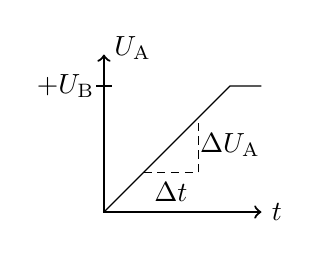
\begin{tikzpicture}
        \draw[thick,->] (-0.015,0) -- (2,0) node[anchor=west] {$t$};
        \draw[thick,->] (0,0) -- (0,2) node[anchor=south west, pos=0.9] {$U_\mathrm{A}$};
        \draw (0,0) -- (1.6,1.6) -- (2,1.6);
        \draw[thick] (-0.1,1.6) -- (0.1,1.6);
        \draw (0,1.6) node[anchor=east] {$+U_\mathrm{B}$};
        
        \draw[densely dashed] (0.5,0.5) -- (1.2,0.5) -- ++(0,0.7);  % Steigungsdreieck Linien
            \node at (1.6,0.85) {$\Delta U_\mathrm{A}$};
            \node at (0.85,0.25) {$\Delta t$}; 
    \end{tikzpicture}
